\label{chap:LiteratureReview}

At the time of writing in 2020, with a  US recession\footnote{This study has not been updated to account for the market crash due to the COVID-19 pandemic.} on the horizon (as shown by data produced by Bloomberg in \autoref{fig:US_recession_prob}), the need for risk assessment is increasingly important to avoid repeating the carnage caused by the 2008 financial crisis. 
While in the past the small and medium (and micro) companies had higher propensity of going bankrupt, more recently we have also seen an uptick in bankruptcies of large global firms. A few examples are the big retail companies such as Toys``R"Us, Debenhams, Forever 21, JC Penney and Sears. The travel agency Thomas Cook and the low-cost airline Flybe have also filed for bankruptcy in the past two years.

% \begin{figure}[htp]
% \centering
% % \captionsetup{justification=centering}
  
%   \centering
%     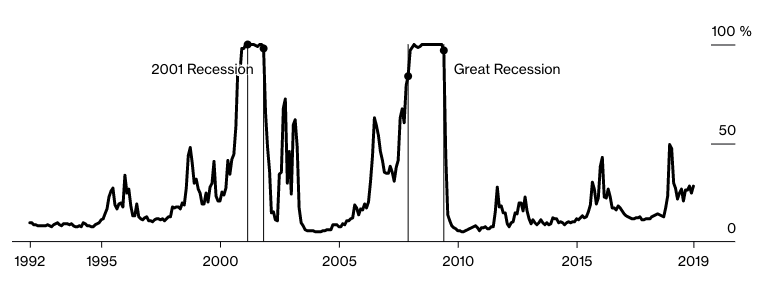
\includegraphics[height=5cm,width=\columnwidth]{Images/recessionUs.png}
%   \caption{Probability of U.S. recession within 12 months. \\
%   Source: \href{https://www.bloomberg.com/graphics/us-economic-recession-tracker/}{Bloomberg}}
%  \label{fig:US_recession}
% \end{figure}
The global recession in 2008 proved that companies were inappropriately evaluated by credit rating agencies and banks. Governments around the world were forced to implement trillion-dollar rescue packages to keep the plumbing behind banking systems running. Given the devastating effects of the financial crisis on firms, now, more than ever, there is a need to identify (and anticipate) upcoming bankruptcies. The surge in the number of research papers around bankruptcy is increasingly evident from \autoref{fig:numberofcases}. 
% During the decade of 2008-2017, the number of publications has increased significantly, representing 83.50\% of total papers analysed. 
% Boosting the accuracy of credit risk and corporate default methodologies used by banks and financial institutions may lead to considerable gains and have a critical impact on global economies. 

% \begin{figure}[htp]
% \centering
% \captionsetup{justification=centering}
  
%   \centering
%     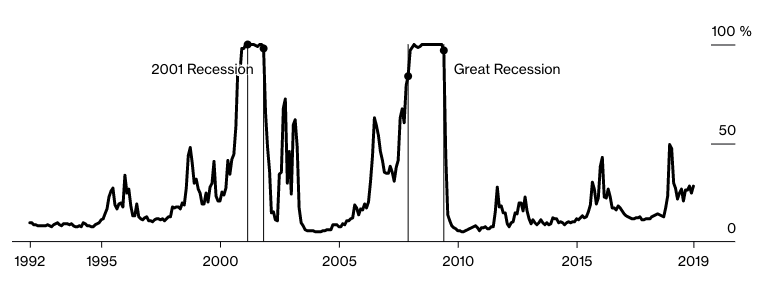
\includegraphics[height=5cm,width=\columnwidth]{Images/recessionUs.png}
%   \caption{Probability of U.S. recession within 12 months. \\
%   Source: \href{https://www.bloomberg.com/graphics/us-economic-recession-tracker/}{Bloomberg}}
%  \label{fig:US_recession}
% \end{figure}

\begin{figure}[htp]
  \centering
%   \captionsetup{justification=centering}
    
      {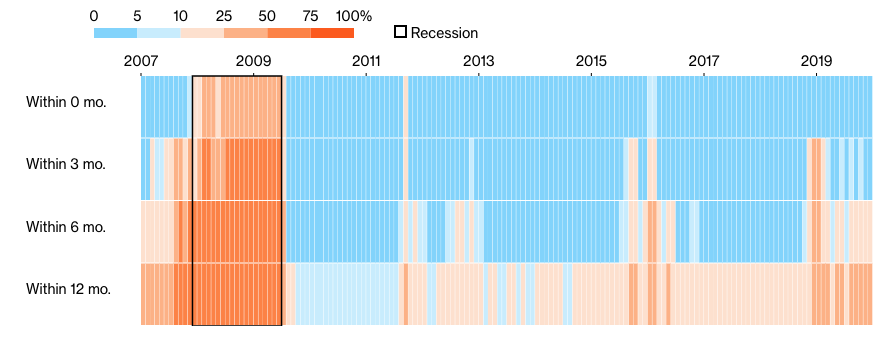
\includegraphics[height=5cm,width=\columnwidth]{Images/recession.png}}
  \caption{Probability of recession within 0, 3, 6 and 12 months \\ 
  Source:\href{https://www.bloomberg.com/graphics/us-economic-recession-tracker/}{Bloomberg}}
  \label{fig:US_recession_prob}
\end{figure}

Situations may arise where a company can become distressed and continue to operate in that condition for many years and can even (at times) recover from their distress. On the other hand, some companies enter bankruptcy immediately after a highly distressing event such as a financial fraud or accounting issues. Several factors influence these outcomes. Lensberg's paper \cite{lensberg2006bankruptcy} investigates related work and categorises numerous factors affecting bankruptcy. Broadly speaking they are audit, financial ratios and fraud indicators, which are measured by qualitative or quantitative variables.
Bankruptcy occurs if a company cannot operate in circumstances, including force majeure events or due to government regulations, or due to its inability to pay off its debt and earn profits for an extended time. 

\begin{figure}[htp]
\centering
% \captionsetup{justification=centering}
  
  \centering
    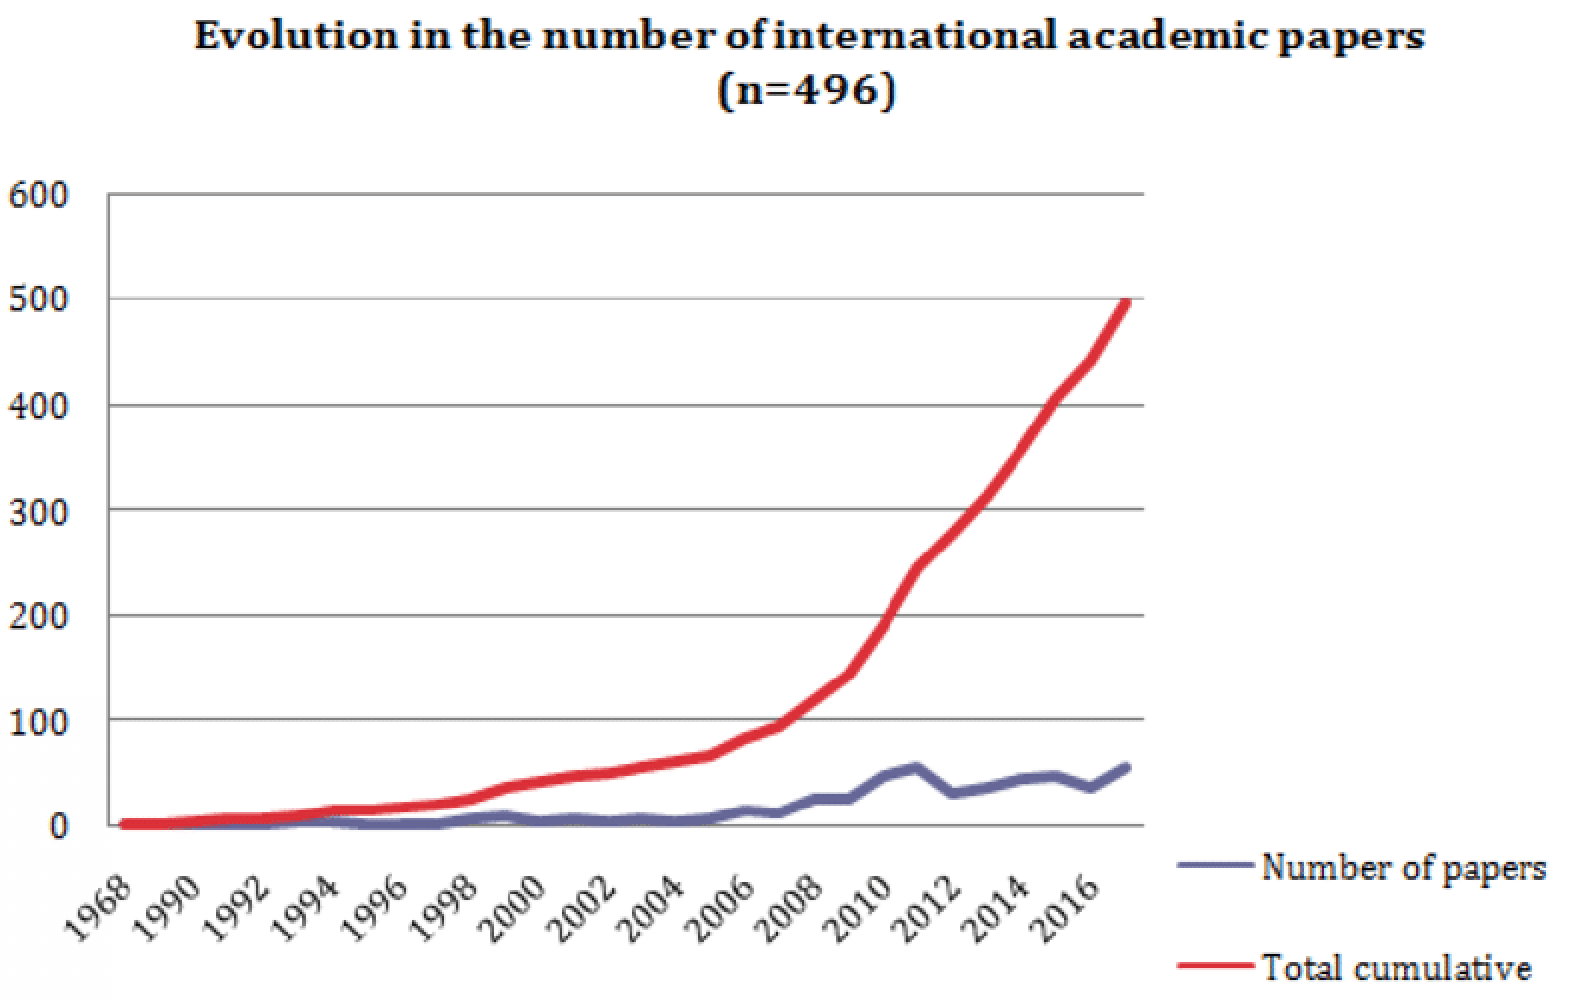
\includegraphics[width=\columnwidth]{Images/evo.png}
  \caption{Rise in the number of international academic articles during the years 1968-2017. This graph has been taken from Shi and Xiaoni's work, published in 2019 \cite{shi2019overview}.}
 \label{fig:numberofcases}
\end{figure}

% Forecasting bankruptcy can be thought of as a classification problem with input variables as the financial, accounting and market data of a firm. Bankruptcy prediction can be stated as a classification problem in the following manner: given a set of parameters (mainly of financial nature) that describe the performance of a company over a given period, what is the probability that the company may become bankrupt during the following year \cite{crone2006impact}.
% Below are some of the reasons for delisting, which can be viewed as de facto bankruptcy: 
% \begin{enumerate}

%     \item Self declaration of bankruptcy/ rehabilitation/ reorganization procedures, 
%     \item Excessive debt
%     \item Suspension of bank transactions, and 
%     \item Termination of business activities (excluding mergers). 
% \end{enumerate}

% In bankruptcy detection, knowing the probability of possible corporate failure is of major importance to all stakeholders since it can help to prevent the adverse effects that such an event can provoke. It is also a key topic related to a measurement of corporate solvency. 
Initial models used in bankruptcy prediction were mainly statistical, such as Multiple Discriminant Analysis \cite{Altman} or Logistic Analysis \cite{ohlson1980financial}. Although these models have been widely used in academia and industry, statistical models are constrained in their ability to increase predictive power. \cite{begley1996bankruptcy}. 
Many recent studies suggest the use of intelligent data mining techniques, including neural networks (NNs), decision trees(DT), case-based reasoning (CBR), support vector machines (SVM), and soft computing \cite{kumar2007bankruptcy}. Neural Networks have an excellent ability to treat non-linear data making them one of the most actively used models in bankruptcy prediction \cite{chandra2010support,baek2003bankruptcy,charalambous2000application}. 

Recent efforts have shown that the performance of predictive models can be significantly enhanced through hybrid and ensemble computing \cite{verikas2010hybrid}. A hybrid system exploits several approaches (e.g., heuristic techniques and classification algorithms) aiming for optimizing the prediction performance. Following this direction, evolutionary algorithms such as genetic algorithm (GA), annealing simulation (AS), particle swarm optimization (PSO), ant colony optimization (ACO), tabu search (TS) are extensively employed in conjunction with machine learning methods \cite{lin2009applying}. The typical usages include tuning the architecture of a particular model (such as the connected weights of MLP \cite{huang2008novel} and the parameters of SVM \cite{min2011tuning}), selecting relevant features, and refining the samples for learning. From another viewpoint, the ensemble approach combines several models and aggregates the output in some rules. It has been shown that a well designed ensemble-based system can outperform a single predictor by inheriting advantages of its base learners.

% \section{Bankruptcy Prediction Models}
% Altman (1968) \cite{Altman} first attempted to simultaneously handle multiple financial ratios. This study used financial data from 33 failed manufacturers, which filed for bankruptcy during 1946– 1965, and that from 33 continuing companies of approximately the same scale. He also manually selected 22 financial indicators that can be classified into seven categories: solvency, profitability, cash flow ratios, capital structure ratios, turnover ratios, growth, and others.

% The classification performances of various combinations among these ratios were examined through a linear discriminant analysis, and five financial ratios were ultimately chosen as effective predictors:

% \begin{enumerate}
%     \item Working capital / Total capital; 
%     \item Retained earnings / Total assets; 
%     \item Earnings before interest and taxes / Total assets;
%     \item Market value of equity interests / Total assets; 
%     \item Amount of sales / Total assets.

% \end{enumerate}


\section{Early Statistical Techniques Used in Bankruptcy Prediction}

The first work using data to predict bankruptcies of companies is from Beaver (1966)\cite{beaver1967financial} and Altman (1968)\cite{Altman}. It appears to be the genesis and benchmark for several empirical studies published henceforth. Beaver \cite{beaver1967financial} developed a one-dimensional dichotomous classification, i.e., based upon a single ratio. Subsequently, Deakin (1972)\cite{deakin1972discriminant} and Edmister (1972)\cite{edmister1972empirical}, have shown that the predictive power of financial ratios is additive and that individual ratios have less predictive power than a small number of independent ratios used simultaneously. The multivariate analysis allows a richer description of the situation of the company and was used systematically.

Shirata (1998) \cite{shirata1998financial} and Taffler (1983) \cite{taffler1983assessment} tried to determine the financial ratios that predict bankruptcy of the company by using only discriminant analysis (DA). However, the new model for predicting the failure inspired by DA such as multi-criteria discriminant analysis was applied by Zopounidis and Doumpos (2002)\cite{zopounidis2002multi}. 
%These latter conclude that this new alternative dominates the DA and that it is a comparative analysis of the logit model.
Subsequently, due to the restrictive statistical requirement of normality for the explanatory variables and quality of the variance-covariance group matrices, logit and probit models were also applied. Among these, the pioneering studies in logistic regression were carried out by Ohlson (1980) \cite{ohlson1980financial}. It is the first in this area to look at the prediction of corporate failure.

West (1985)\cite{west1985factor} used the factor analysis to create composite variables to describe a bank’s financial and operating characteristics. Experimental results demonstrated that the combined method of factor analysis and logit was promising for evaluating the bank's condition.
However, these conventional statistical techniques have some restrictive assumptions, such as the linearity, normality, independence among predictor variables and pre-existing functional form relating the criterion variable and the predictor variable. 

In more current literature, when predicting corporate bankruptcy, researchers have routinely used accounting-based variables (e.g., profitability ratio and liability ratios) and market-based variables (e.g., stock market returns and volatility) as a gauge of default risk. We refer readers to Kumar and Ravi's paper \cite{kumar2007bankruptcy}  that provides a comprehensive literature review on the studies before 2008. In \autoref{tab:Recent_studies_on_bankruptcy_prediction}, we curate a list of more recent studies on bankruptcy prediction. 

\newpage
% \todo[inline]{Fix formatting}
\begin{center}
\small
% \begin{sc}
\begin{longtable}{|p{2.5cm}|p{2.5cm}|p{1.2cm}|p{3.5cm}|p{2cm}|p{2cm}|}

\hline
 Study  & Source of data & Sample size & Models & Time period & Variables type   \\ [0.5ex] 
\hline\hline

    Sueyoshi and Goto (2009)\cite{sueyoshi2009dea} & Japanese Construction Industry & 1K & DEA-DA, PCA & 2000–2005 & Accounting \\ \hline
    
    Ioannidis, Pasiouras, and Zopounidis (2010)\cite{ioannidis2010assessing} \cite{ioannidis2010assessing} & 78 countries, Bankscope, World Bank & 1K & UTADIS, MLP, CART, KNN, Ordered logit, stacked models & 2007–2008 & Accounting, country-level variables \\ \hline
    
    Chen et al. (2011)\cite{chen2011genetic} & France, Diane database & 1K & GA + LVQ & 2006–2007 & Accounting \\ \hline
    
    Olson, Delen, and Meng (2012)\cite{olson2012comparative} & USA, Compustat & 1K & DT, logit, MLP, RBFN, SVM & 2005–2009 & Accounting \\ \hline
    
    Ding et al. (2012)\cite{ding2012class} & USA, Compustat, CRSP & 1M+ & Transformation Survival Model & 1981–2006 & Accounting \& Market \\ \hline
    
    Sánchez-Lasheras et al. (2012)\cite{sanchez2012hybrid} & Spain, Bureau van Dijk & 63K & SOM + MARS & 2007–2008 & Accounting (5 Altman variables) \\ \hline
    
    Cinca and Nieto (2013)\cite{serrano2013partial} & USA, FDIC & 8K & PLS-DA & 2008–2011 & Accounting \\ \hline
    
    Geng et al. (2015)\cite{geng2015prediction}& China, CSMAR & 200 & NN, DT, SVM, MV & 2001–2008 & Accounting \\ \hline
    
    Wanke et al. (2015)\cite{wanke2015financial} & Brazilian, Economatica & 600 & DEA+DSBM & 1996–2011 & Accounting \\ \hline
    
    du Jardin (2015)\cite{du2015bankruptcy} & France, Bureau van Dijk – Diane database & 18K & DA, logit, MLP, SA & 2003–2012 & Accounting \\ \hline
    
    Tian et al. (2015)\cite{tian2015variable} & USA, Compustat, CRSP & 1.5M & Discrete Hazard Model, Logit & 1980–2009 & Accounting \& Market \\ \hline
    
    du Jardin (2016)\cite{du2016two} & France, Bureau van Dijk – Diane database & 17K & Bagging, boosting, random subspace, PBM & 2003–2012 & Accounting \\ \hline
    
    Liang et al. (2016)\cite{liang2016financial} & Taiwan Economic Journal (TEJ) & 500 & SVM, KNN, NB, CART, MLP & 1999–2009 & Accounting, market, corporate governance \\ \hline
    
    Doumpos et al. (2017)\cite{doumpos2017corporate} & 18 EU countries, Bureau van Dijk, Eurostat, IEA, OECD, and UNECE & 13K & MCDA & 2012–2016 & Accounting, Macroeconomic, energy markets \\ \hline
    
    Calabrese et al. (2017)\cite{calabrese2017effectiveness} & U.S. Department of the Treasury, FDIC, Call Reports & 10K & LOBGEV(GEV model and D-vine copula) & 2008–2013 & Combination of variables \\ 
\hline
    

\caption{Recent studies on bankruptcy prediction.} 
\label{tab:Recent_studies_on_bankruptcy_prediction} 
\end{longtable}
% \end{sc}
\end{center}

\section{Recent Intelligent Techniques in Bankruptcy Prediction} 
In recent years, many studies have demonstrated that intelligent techniques can be alternate methodologies to predict corporate bankruptcy. Intelligent techniques automatically extract knowledge from a dataset and construct different model representations to explain the data set. The major difference between intelligent techniques and statistical techniques is that statistical techniques usually need researchers to impose structures to different models, such as linearity in the multiple regression analysis. Statistical techniques also require researches to construct the model by estimating parameters to fit the data or observation, while intelligent techniques allow learning the particular structure of the model from the data \cite{wang2011comparative}.

Most of the studies in \autoref{tab:Recent_studies_on_bankruptcy_prediction} fall into the intelligent technique category. The goal of these studies was to develop accurate models using artificial intelligence and operations research techniques. Also, models that allow non-linear decision boundaries (e.g., neural networks, SVM with non-linear kernels) quickly gained popularity and are now widely applied. These features provide better model flexibility and improved classification performance. A trend in recent literature is studying the combinations of models. Several studies demonstrate how to combine various models horizontally using ensemble techniques as shown by Geng et al (2015) \cite{geng2015prediction} and Kim \& Kang, (2010)\cite{kim2010ensemble}, or vertically as shown by du Jardin (2016) \cite{du2016two}. These hybrid models can capture greater variations in the decision space and result in more stable and accurate predictions.

Second, we notice a wide diversification of data sources in recent studies. As noted before, theoretical and empirical studies have long established that accounting-based ratios and market-based variables are the main indicators of future bankruptcy. More recent studies have started to evaluate the predictive power of data sources beyond the two types of variables. For example, Liang, Lu, Tsai, and Shih (2016)  \cite{liang2016financial} examines the discriminatory power of a broad array of corporate governance indicators (discussed in detail in \autoref{sec:CGI}), including board structure, ownership structure, leadership personnel, and others. Doumpos, Andriosopoulos, Galariotis, Makridou, and Zopounidis (2017)’s model \cite{doumpos2017corporate} takes country characteristics into account. They show that country-level data on the economic and business environment, energy efficiency policies, as well as characteristics of markets, can add value to corporate failure prediction models. Calabrese, Degl'Innocenti, and Osmetti (2017) \cite{calabrese2017effectiveness} study how the U.S. government's Troubled Asset Relief Program (TARP) impacted the probability of failure among commercial banks. 
% Examining the effectiveness of these new data sources can expand the scope of features selections for prediction models and offer policy prescriptions.


% This review covers the intelligent techniques concluded in the studies belonging to
% (i) different neural network (NN) architectures including multi-layer perception (MLP), probabilistic neural networks (PNN), auto-associative neural network (AANN),
% (ii) decision trees, 
% (iii) case-based reasoning,
% (iv) evolutionary approaches and
% vii) operational research techniques including linear programming (LP), data evelopment analysis (DEA).
\autoref{table:intelligent_techniques} provides an overview of some of the other machine learning algorithms used in past studies. The models used in our research are discussed in greater detail in \autoref{chap:Methodologies}.

\begin{table}
\small
\begin{center}
 \begin{tabular}{|p{0.5cm}|p{2cm}|p{3.75cm}|p{3.75cm}|p{3.75cm}|} 
 \hline
 S/N & Variable  & Description & Advantages & Disadvantages   \\ [0.5ex] 
 \hline\hline

    1. & Neural Networks (NN) & Learn from examples using several constructs and algorithms just like a human being learns new things & Good at function approximation, forecasting, classification, clustering and optimization tasks depending on the neural network architecture & The determination of various parameters associated with training algorithms is not straightforward. Many neural network architectures need a lot of training data and training cycles (iterations) \\ \hline
    
    2. & Genetic Algorithms (GA) & Mimics Darwinian principles of evolution to solve highly nonlinear, non-convex global optimization problems & Good at finding the global optimum of a highly nonlinear, non-convex function without getting trapped in local minima & Does take a long time to converge; May did not yield global optimal solution always unless it is augmented by a suitable direct search method \\ \hline
    
    3. & Case-based reasoning (CBR) & Learns from examples using the euclidean distance and k-nearest neighbour method & Good for small data sets and when the data appears as cases; similar to the human-like decision-making & Cannot be applied to large data sets; poor in generalization \\ \hline
    
    4. & SVM & It uses statistical learning theory to perform classification and regression tasks & It yields global optimal solution as the problem gets converted to a quadratic programming problem; It can work well with few samples & Selection of the kernel and its parameters is a tricky issue. It is abysmally slow in the test phase. It has high algorithmic complexity and requires extensive memory \\ \hline
    
    5. & Rough sets & They use a lower and upper approximation of a concept to model uncertainty in the data & They yield `if-then’ rules involving ordinal values to perform classification tasks & It can be (a) sometimes impractical to apply as it may lead to an empty set (b) sensitive to changes in data and (c) inaccurate \\ 

\hline
\end{tabular}
\end{center}

    \caption{Merits and Demerits of Intelligent Techniques.}
\label{table:intelligent_techniques}
\end{table}

\section{Corporate Governance Indicators}
\label{sec:CGI}
The general definition of corporate governance includes the mechanisms, processes and relations by which corporations are controlled and directed \cite{shailer2004introduction}. 
% An integrated set of internal and external control mechanisms allow shareholders to exercise appropriate oversight of a company to maximize firm value and ensure that it generates a return on their holdings \cite{chen2014financial}.

Many corporate governance indicators (CGIs) have been identified in the literature which has been used for solving bankruptcy or financial crisis problems. These can be broadly classified into five categories including board structure, ownership structure, cash flow rights, key persons retained, and others. 
% However, not all the CGIs used for predicting bankruptcy in related works are the same. In other words, different categories of CGIs have been considered in different studies.

However, the prediction performance obtained by combining CGIs and financial ratios has not been fully examined. Only some selected CGIs and financial ratios have been used in related studies and the chosen features may differ from study to study. 
Lee (2004) \cite{lee2004corporate} uses six financial ratios belonging to solvency, profitability, and other categories use. It also uses ten CGIs in the board structure and ownership categories. They found that model performance was enhanced by using a combination of CGIs and financial ratios.
%   According to \cite{liang2016financial}, where the CGIs of board structure, ownership structure, cash flow rights, retention of key personnel, and others are analysed on a real-world dataset from Taiwan. Results show that the FR categories of solvency and profitability and the CGI categories of board structure and ownership structure are the most important features in bankruptcy prediction. 
% Specifically, the best prediction model performance is obtained with a combination in terms of prediction accuracy, Type I/II errors, ROC curve, and misclassification cost. 
However, these findings may not be applicable in some markets where the definition of distressed companies is unclear and the characteristics of corporate governance indicators are not obvious, such as in the Chinese market.
 
\textbf{Note:} Although including CGI data in our research would be very promising, the paucity of such data hinders our ability to incorporate CGIs into our bankruptcy prediction models.

\section{Ensemble Classifiers in Bankruptcy Prediction}
Ensemble methods have been known to be used as tools to improve the accuracy of learning algorithms by combining a set of weak classifiers (otherwise called weak learners), each of which needs only moderate performance on the training set \cite{perrone1994putting,schapire1990strength}. Two popular methods for creating accurate ensembles are Bagging \cite{breiman1996bagging} and Boosting \cite{freund1996experiments}. Both theoretical and empirical studies have demonstrated remarkable improvements in the generalisation behaviour \cite{bauer1999empirical,friedman2000additive}. Literature suggests that ensemble methods decrease the generalisation error of CART decision trees \cite{breiman1996bagging}, C4.5 decision trees \cite{quinlan1987simplifying}, and Neural Networks (NNs) \cite{opitz1999popular}.

Several studies on the bankruptcy prediction have applied AdaBoost, a popularly used boosting algorithm, to bankruptcy classification. Results have shown that AdaBoost decreases the generalisation error and improves the accuracy \cite{cortes2007multiclass} of these ensemble classifiers. An empirical comparison has shown that AdaBoost with classification trees decreases the generalisation error by around 30\%  with respect to an error produced with a NNs \cite{alfaro2008bankruptcy}. 
Previous studies have suggested that ensembles with classification trees are very effective for bankruptcy prediction, however, there has been little empirical testing of an ensemble with NNs in bankruptcy prediction literature. The primary reason is that ensembles with decision trees provide fast training speed and well-established default parameter settings, while NNs has the difficulties for testing both in terms of the significant processing time required and in selecting training parameters \cite{opitz1999popular}.
The significant overhead in training NNs and its hyper-parameter optimisation is the main reason that we exclude NNs from our comparative study.

We choose to use ensemble methods as they are expected to provide the following advantages over the traditional NNs (as detailed in \cite{kim2010ensemble}); 
First, ensembles have been shown to produce results with greater prediction performance compared to any of the individual NNs classifiers.
Second, the classification approaches that use error minimisation are prone to overfitting when a classifier is highly adjusted to learn the training set. This causes the classifier’s generalisation error to increase significantly when it is applied to previously unseen data. 
Ensemble models like Random Forests, Bagging and XGBoost are robust to overfitting and thus reduce generalisation error. 
% Finally, ensembles with a variety of standard classifiers is expected to provide further insight into the general characteristics of ensemble methods which are influenced by the learning algorithm.

Against these backgrounds, we propose three ensemble methods to improve the performance of bankruptcy prediction. The three popular methods, Random Forests, Bagging and Extreme Gradient Boosting (XGBoost), are used for creating high-performance ensembles by combining the predictions of multiple tree-based (weak) classifiers. This paper presents a comprehensive evaluation of applying these ensemble models on predicting bankruptcy of listed Japanese firms.

Our review of the bankruptcy prediction literature has highlighted three key gaps. First, there is a lack of seminal work done on Japanese financial data. This gives an opportunity to put forth our analysis on this seldomly studied economy. Second and to the best of our knowledge, a comprehensive comparison regarding data imputation models on financial data and their effect on the performance of bankruptcy prediction models have not been undertaken on financial data from Asia.
Third, a holistic performance evaluation of tree-based ensemble models, specifically Random Forests, Bagging and XGBoost on the Japanese Data has not been conducted before, but similar studies on leading economies such as USA, France and Germany have yielded positive performance results. We aim to help address these important gaps in the literature.



